\chapter{Estado del arte}
\label{ch:estado_del_arte}

Como se ha explicado en la \hyperref[ch:introduccion]{introducción}, este trabajo continúa el comenzado por el alumno Rubén Sanchez en cursos anteriores. Por ello, el primer paso a realizar como revisión del estado del arte es una ingeniería inversa de su desarrollo, con el fin de identificar aspectos en los que se puede mejorar.

\section{Ingeniería inversa}
\label{sec:inginv}

Al comenzar el trabajo, se recibe por parte del tutor el prototipo del dispositivo, que se puede ver en las figuras \ref{fig:pwmbox_top} y \ref{fig:pwmbox_side}.

\begin{figure}[h!]
    \centering
    \includegraphics[width=\textwidth]{pwmbox_top.jpg}
    \caption{Dispositivo PWM Box desde arriba.}
    \label{fig:pwmbox_top}
\end{figure}

\begin{figure}[h!]
    \centering
    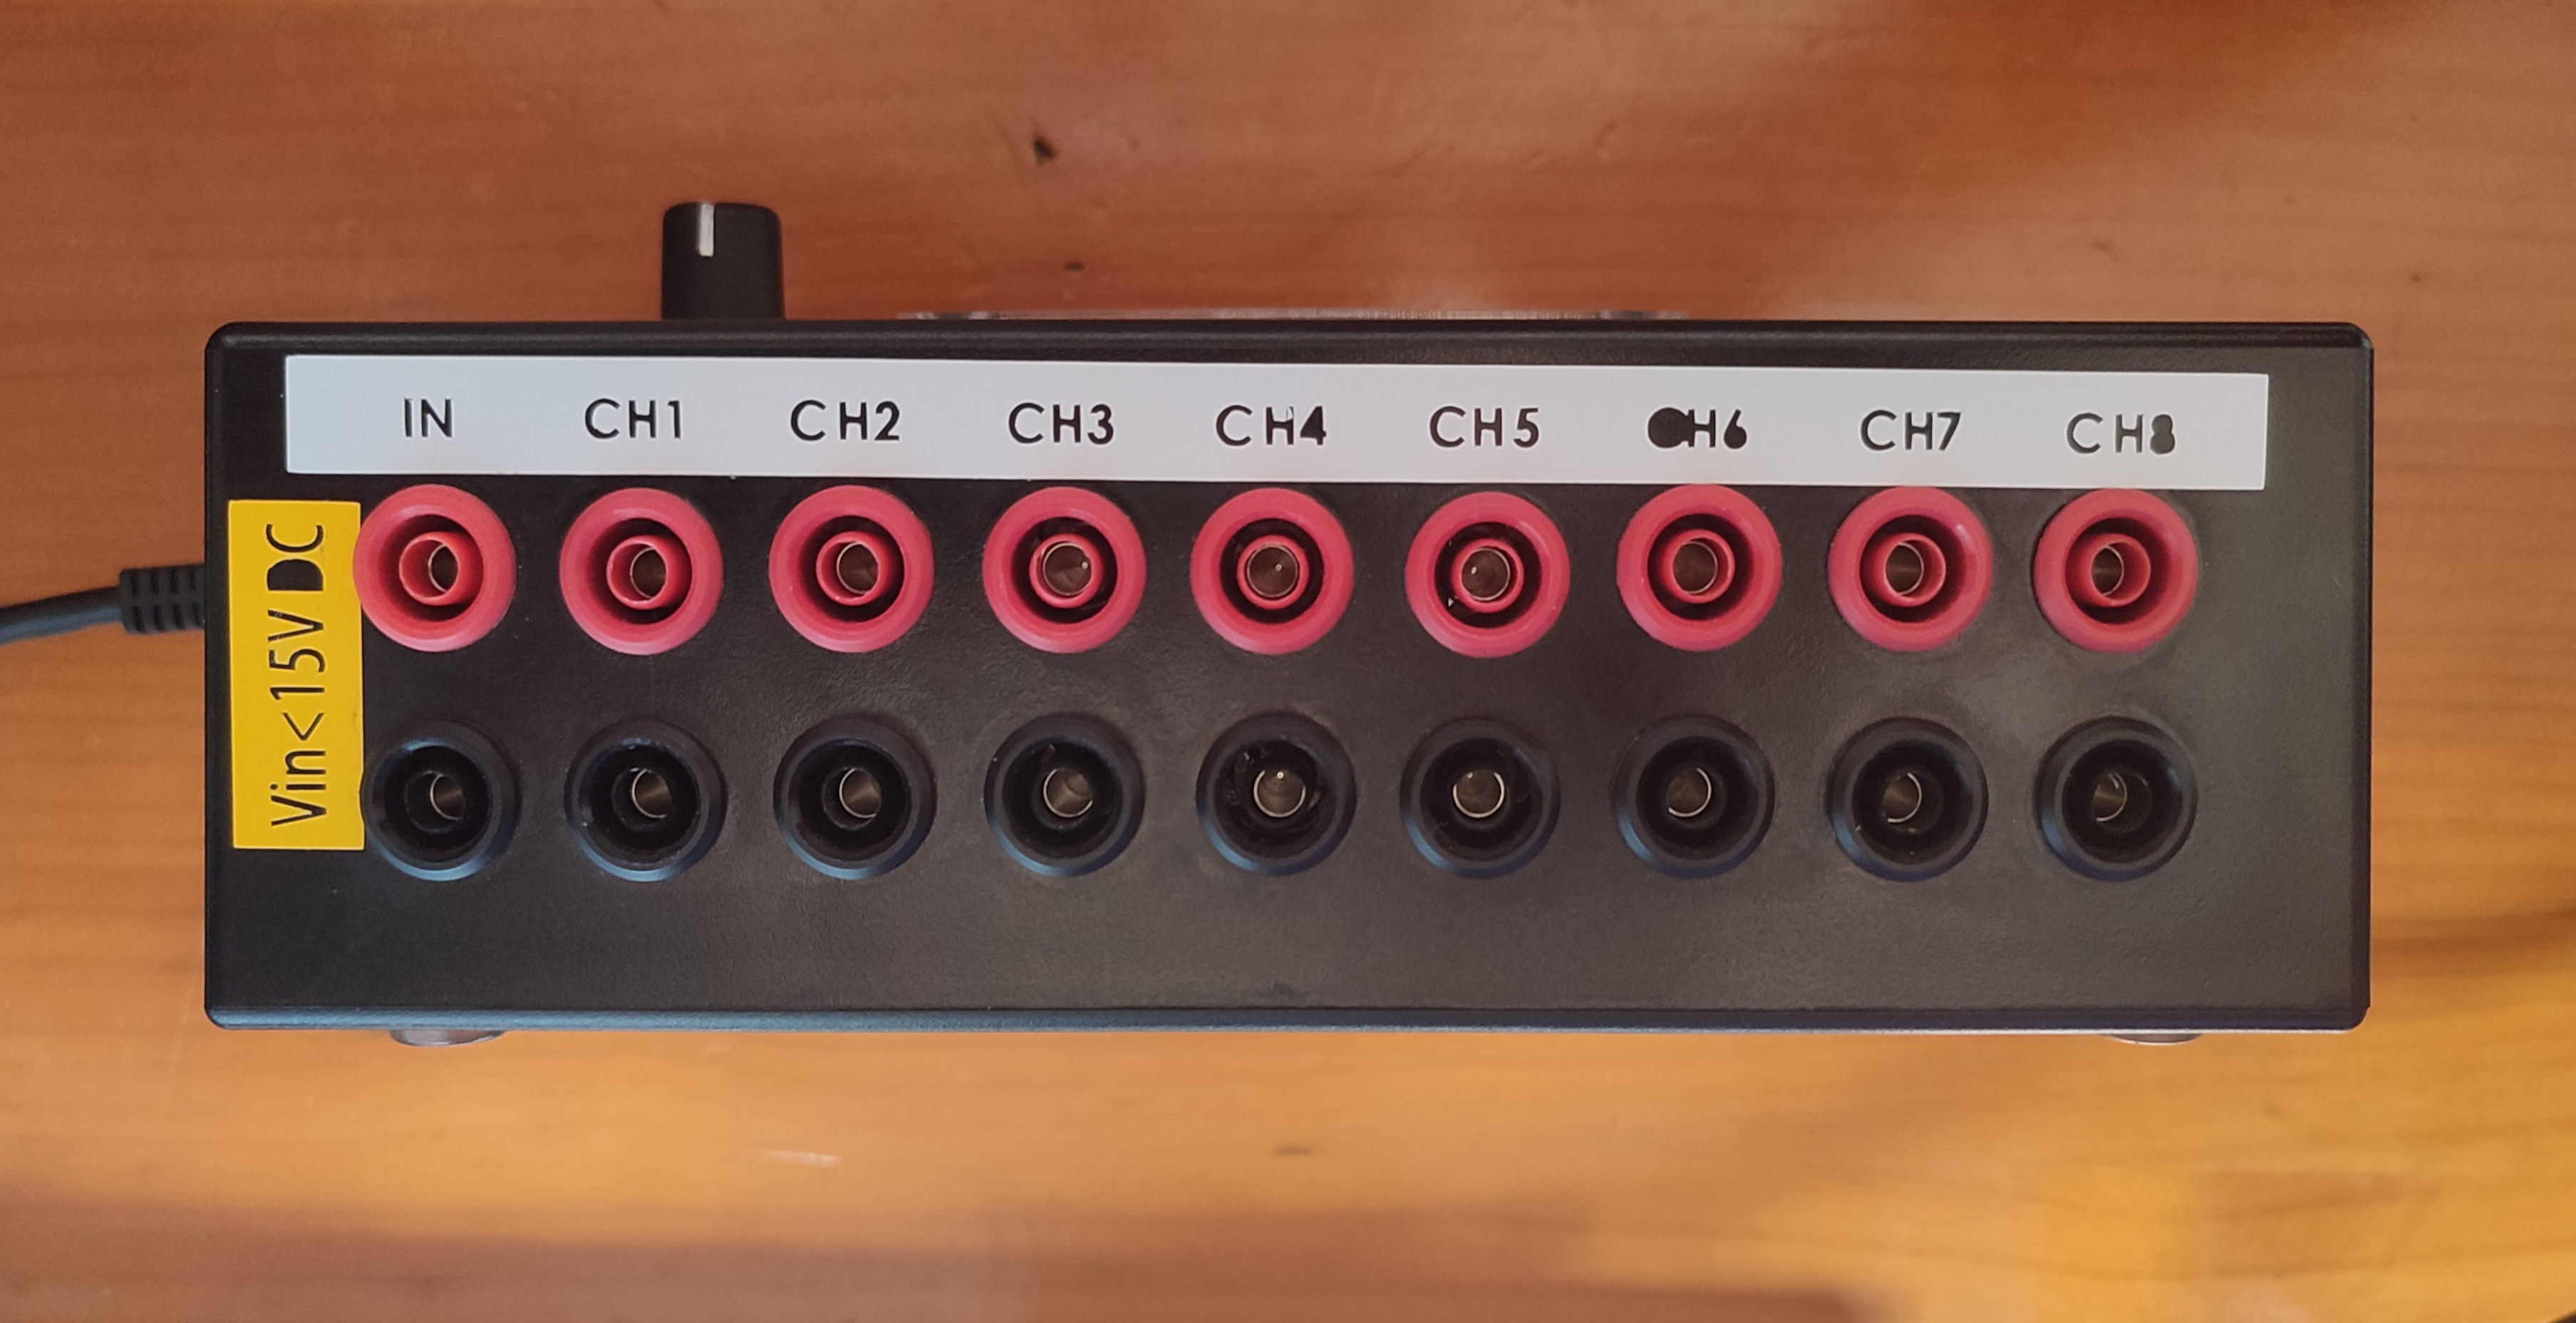
\includegraphics[width=\textwidth]{pwmbox_side.jpg}
    \caption{Lateral del dispositivo PWM Box.}
    \label{fig:pwmbox_side}
\end{figure}

Este está compuesto por un Arduino Mega 2560, una pantalla LCD de 4 líneas, un \textit{rotary encoder} y 8 conectores de salida. Por cada uno de estos 8 conectores se produce una salida PWM cuyos parámetros (encencido, frecuencia, ciclo de trabajo y fase) pueden ser configurados por el usuario, pensada para conectar y probar los distintos modos del faro del vehículo.

Por otro lado, se recibe un archivo comprimido que contiene el código existente del proyecto, así como alguna documentación escrita por sus previos contribuyentes. Estos archivos se muestran en la figura \ref{fig:fw_v0}.

\begin{figure}[ht]
    \centering
    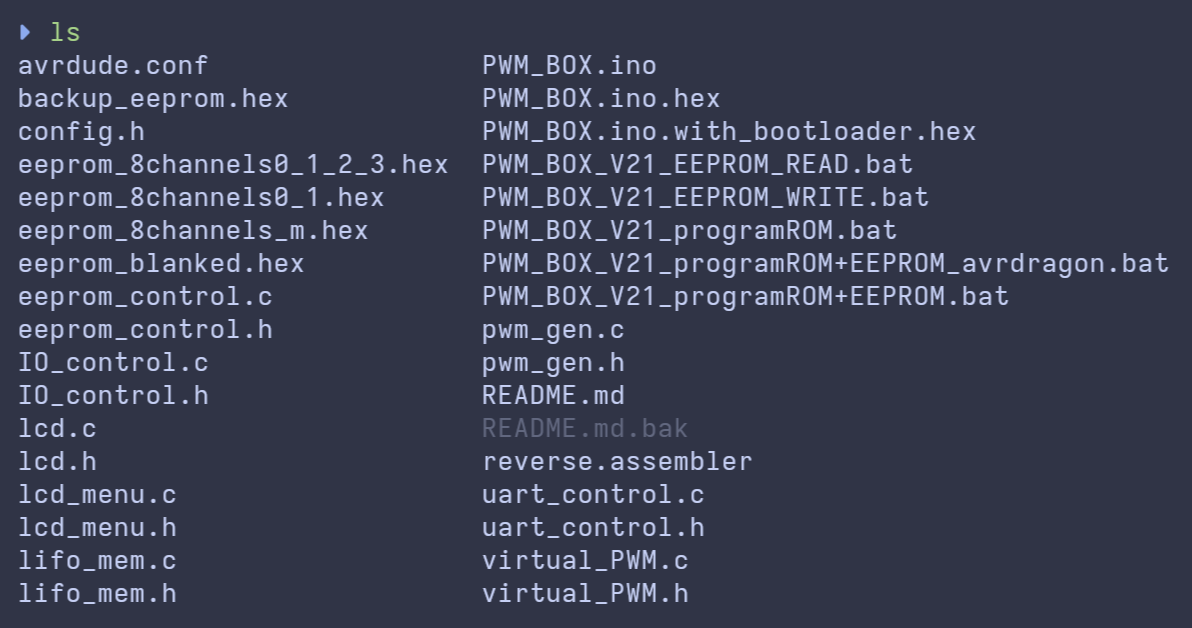
\includegraphics[width=0.8\textwidth]{fw_files_v0.png}
    \caption{Contenido de \textit{PWM\_BOX.RAR}.}
    \label{fig:fw_v0}
\end{figure}

Con esto, se procede a realizar una clasificación básica de los distintos ficheros a modo de primera toma de contacto con el proyecto. Según su contenido y utilidad, se pueden distinguir los siguientes tipos de archivos:

\begin{itemize}
    \item{\textbf{Archivos HEX:}} Estos contienen datos en formato hexadecimal. Por el nombre, se pueden distinguir entre los que contienen datos para la memoria no volátil del microcontrolador (EEPROM), y los que contienen el programa en sí.
    \item{\textbf{Archivos BAT:}} Se tratan de archivos de comandos para Windows. Examinando su contenido, se puede ver que todos ellos ejecutan comandos de un programa llamado AVRDUDE.\\
    AVRDUDE es una utilidad multiplataforma para la programación de microcontroladores AVR, entre los que se encuentran los usados por Arduino. Permite todo tipo de operaciones de carga y descarga de datos de las distintas memorias del microcontrolador. Es una herramienta usada muy comúnmente, funcionando incluso de \textit{back-end} en otros entornos de desarrollo.
    \item{\textbf{Archivos de código:}} Por un lado tendríamos las cabeceras y su implementación, en los usuales archivos H y C. Por otro lado, encontramos un archivo INO, que es el tipo usado por Arduino IDE para distinguir que se trata del archivo principal del proyecto. Este contiene las funciones \verb|setup()| y \verb|loop()|, que definen el flujo básico del programa: la primera se ejecuta una vez al inicio, y la segunda conforma el bucle principal de ejecución.
\end{itemize}

Tras esta primera distinción, se pasa a hacer un análisis del código y de su funcionamiento, usando como apoyo la documentación de Rubén. Según la misma, se puede dividir el programa en los grupos que se describen a continuación.

\subsection{Archivo principal}

Consiste en el archivo principal INO que se mencionó anteriormente. En él, encontramos algunos elementos usados para determinar el flujo de ejecución del programa:

\begin{itemize}
    \item En primer lugar tenemos una cola de eventos, que recoje las acciones del usuario y permite al programa procesarlas en orden. Se desarrollará en una sección posterior.
    \item Un contador de tiempo, que mide cuánto lleva el usuario sin interactuar con el dispositivo para mostrar u ocultar un salvapantallas.
    \item El uso de distintas interrupciones para el manejo de la entrada del usuario, la generación de la señal PWM de salida y la comunicación por UART. \end{itemize}

Una cosa a comentar sobre el actual flujo del programa es el uso de interrupciones. Su uso es muy necesario para la generación de las señales PWM. Una interrupción se genera a una cierta frecuencia, y, dependiendo de los parámetros que introduzca el usuario, las señales cambian de estado cuando les corresponda. Esto asegura que los cambios se realizan en el momento preciso, mientras que si se gestionaran en el bucle principal, el momento exacto de las actualizaciones sería más incierto.

Sin embargo, la alta frecuencia de las interrupciones podría provocar una ``sobrecarga'' (\textit{interrupt overload}). Esta provocaría que otras tareas en ejecución, en este caso el bucle principal, no recibiera el suficiente tiempo de CPU, afectando al rendimiento. Esta condición puede también darse si, aun manteniendo un bajo número de interrupciones, las rutinas que estas ejecutan son demasiado largas.

Por todo ello, el uso de interrupciones para manejar la entrada de usuario a través del codificador rotatorio parece, tras un primer análisis, acertado. Su frecuencia será varias magnitudes menor que las destinadas a atender las señales de salida, de forma que no aportarán al problema anteriormente mencionado. Al mismo tiempo, se asegurarán de que ningún \textit{input} del usuario se pierde debido a que la CPU se encuentre ocupada. \cite{chapman}

\subsubsection{Buffer de eventos} Se trata de una cola circular estándar, en la que se van incluyendo datos de tipo evento. Estos consisten de un entero que determina el tipo de evento, junto a dos parámetros opcionales. Estos últimos parecen no ser utilizados en el resto del programa. Se distinguen eventos para giros del \textit{rotary encoder}, para su pulsación y para la llegada de datos a la UART.

El uso de un buffer de eventos aporta un mecanismo más para evitar la comentada sobrecarga por interrupciones. Con él, las funciones que las procesan pueden dedicarse únicamente a añadir el evento que corresponda a la cola, evitando rutinas demasiado largas. Será luego el bucle principal el que se encargue de ejecutar la acción vinculada al evento concreto, cuando la CPU pueda dedicarle tiempo.

\subsection{EEPROM}

Se trata de un archivo que sienta las bases para el guardado de datos en la memoria no volátil del microcontrolador. Este punto se distingue como uno de los que quedó fuera del desarrollo anterior, ya que únicamente aparecen implementadas algunas funciones básicas para leer posiciones determinadas de la memoria, que llaman directamente a otras de la librería de AVR.

De la breve implementación presente en este punto se puede comentar una cosa, y es que las lecturas y escrituras se están realizando proporcionando directamente la posición de memoria. Esto es un claro punto a mejorar, puesto que mantener estas posiciones guardadas puede ser tedioso, y disminuir la legibilidad del código. Una forma más apropiada de tratarlo sería definir la estructura de la memoria, de forma que los accesos a la misma puedan realizarse usando variables.

\subsection{Entrada/Salida}

En él se definen distintas funciones relacionadas con el codificador rotatorio y el manejo de eventos. También se distingue el prototipo de una función que serviría para decodificar un mensaje recibido por el puerto serie. Sin embargo, la lógica a bajo nivel del mismo no está implementada, por lo que actualmente no se le está dando uso.

De este módulo cabe destacar que el funcionamiento del \textit{rotary encoder} no es del todo correcto, generando en ocasiones dobles pulsaciones y no detectando algunos de los giros.

\subsection{LCD}

Se trata, con diferencia, del módulo más extenso de todo el programa. En él aparecen definidas distintas funciones que determinan el contenido de la pantalla según las acciones que vaya realizando el usuario. Podemos distinguir los siguientes menús:

\begin{itemize}
    \item\textbf{Lista:} Es el menú principal del sistema. En él se muestran las diferentes señales a configurar, así como las opciones de guardar y cargar configuraciones en la EEPROM (no operativas aún).
    \item\textbf{PWM:} Permite la configuración de los 4 parámetros principales del PWM que se seleccione en la pantalla anterior.
    \item\textbf{Contraseña:} Permite bloquear algunas características del dispositivo, como las que alteran el estado de la memoria EEPROM, tras una contraseña, evitando el acceso de usuarios no autorizados.
\end{itemize}

Para cada uno de los menús mencionados, se encuentran en este archivo las definiciones de cuatro funciones, que permiten realizar operaciones básicas sobre el menú al que pertenecen. Se tratan de las siguientes:

\begin{itemize}
    \item\textbf{Actualización de la pantalla:} Encontramos una para cada menú del firmware. Se encarga de dibujar el contenido del LCD dependiendo del contexto, como el lugar en el que se encuentre el cursor, la opción que se encuentre activa, etc.
    \item\textbf{Pulsación del botón:} Determina la acción a realizar cuando el usuario accione el \textit{rotary encoder}, basándose una vez más en la posición del cursor.
    \item\textbf{Desplazamiento hacia arriba:} Concreta el cambio a realizar en las variables internas del menú cuando el usuario gire el control hacia la izquierda.
    \item\textbf{Desplazamiento hacia abajo:} Realiza la misma función que el punto anterior, pero para un giro en la dirección opuesta.
\end{itemize}

De esta parte se extraen varios puntos a mejorar. Por un lado, el archivo es demasiado extenso como para ser navegado cómodamente. Contiene la implementación de todas las funciones de todos los menús del sistema sin demasiada organización, incluso aunque durante la ejecución sólo se usen en cada momento las del menú que se encuentre activo. De la misma forma, como se ha señalado de manera consciente, encontramos código redundante dentro de las funciones de un mismo menú, como pone de manifiesto manejar las dos direcciones de giro del \textit{rotary encoder} en funciones separadas.

Por otro lado, las variables que hacen referencia a los distintos menús se encuentran agrupadas en estructuras independientes. De esta forma se consigue que no haya conflicto entre ellas, pero hacen el código mucho menos legible debido a la longitud de cada una de sus referencias.

Esto trae consigo numerosos problemas que dificultan el mantenimiento del código, tanto a la hora de corregir errores existentes como al tratar de extender las funcionalidades del dispositivo, que son dos de los \hyperref[sec:objetivos]{objetivos} de este trabajo.

Adicionalmente, se ha detectado el incorrecto funcionamiento del \textit{rotary encoder} en determinados menús, en los que las direcciones de giro están invertidas.

\subsection{Vista general}

Esta versión del firmware establece una buena base para el desarrollo. Define un flujo de ejecución sólido, y nos permite centrar los esfuerzos en realizar las correciones y mejoras oportunas sobre los distintos módulos de manera individual. De esta forma, se divide el trabajo en objetivos concretos que evitan grandes modificaciones que no sean estrictamente necesarias, así como consecuentes inversiones innecesarias de tiempo.

A su vez, de manera global, se han detectado en el código algunos puntos a mejorar en cuanto a legibilidad, presentación y usabilidad del código. Sin embargo, este es un aspecto subjetivo, por lo que no se cubrirá en esta memoria.

\section{Tecnologías usadas}

En esta sección destacaré las distintas herramientas y tecnologías involucradas en el desarrollo del proyecto, aportando algunas posibles alternativas y destacando la opción elegida en cada caso.

\subsection{Sistema operativo}

Hasta ahora, todo el código usado en el proyecto se ha desarrollado en Windows. Dada la necesidad de comprobar el funcionamiento del producto final tanto en este como en Linux (establecida como objetivo en la sección \hyperref[sec:objetivos]{Objetivos}), el sistema operativo a usar no es un aspecto decisivo a tener en cuenta en este caso. Al fin y al cabo, todo el software que se utilice ha de ser compatible con ambos.

Sin embargo, en este caso, se ha decidido usar Linux por preferencia personal. Esto puede resultar un inconveniente a la hora de usar los archivos BAT proporcionados al comienzo del proyecto. Sin embargo, como se comentó en la sección anterior, el programa al que estos hacen referencia es multiplataforma, por lo que bastaría con transferirlos a un \textit{script} en Bash si fuese necesario.

En general, al no ser algo relevante en el proyecto, consideramos que la familiaridad con el entorno de desarrollo resulta una prioridad, debido a la capacidad que proporciona para solucionar cualquier imprevisto que pueda surgir en el curso del trabajo. A la hora de probar el código, se puede recurrir a una máquina virtual, o a una partición con otro sistema si se prefiere.

\subsection{Lenguajes de programación}

\subsubsection{Firmware}

El lenguaje de programación usado actualmente en el proyecto es C. C es un lenguaje de programación de propósito general diseñado originalmente para su uso en el sistema operativo UNIX, estando este, junto a la mayoría de programas usados en él, escritos en C. Sin embargo, su uso a lo largo del tiempo ha transcendido su objetivo inicial, convirtiéndose en un lenguaje muy ampliamente usado en la actualidad, debido entre otros factores a la eficiencia del código que produce y a su portabilidad. Dispone de estructuras típicas de los lenguajes de alto nivel, permitiendo a su vez un gran control del sistema a bajo nivel. Esto lo convierte en un lenguaje muy versátil, pudiendo llegar a ser más conveniente y efectivo en la ejecución de diversas tareas que otras alternativas más potentes. \cite{k&r}

Estando esta parte del proyecto basada en la programación de un Arduino, la otra opción disponible sería usar C++. Este surgió con la intención de extender el lenguaje de programación C a través de la inclusión de características de la programación orientada a objetos. A lo largo del tiempo, se fueron también incorporando a él otras funciones propias de la programación genérica, de la programación estructurada, facilidades para la programación a bajo nivel... Es por ello que se suele considerar a C++ un lenguaje de programación multiparadigma. C++ es un lenguaje muy completo, manteniendo la eficiencia de C pero añadiendo un gran número de características de lenguajes de más alto nivel, siendo apropiado para el desarrollo de programas, videojuegos o servidores.

Teniendo en cuenta que el objetivo actual de este ámbito es añadir algunas características y pulir la implementación del firmware, se considera más apropiado continuar trabajando en el lenguaje con el que se empezó el proyecto, es decir, C. 

\subsubsection{Interfaz}

Para el desarrollo de la interfaz se necesita una librería gráfica que sea compatible tanto con Windows como con Linux, dado uno de los \hyperref[sec:objetivos]{objetivos} definidos anteriormente. Debido a ello, así como a experiencias previas, se ha optado por el uso de Qt.

Qt se trata de un \textit{framework} multiplataforma que permite la creación de interfaces gráficas compatibles con Linux, Windows, macOS, Android y otros sistemas empotrados sin necesidad de modificar el código base. Qt proporciona licencias comerciales, pero también está disponible como código abierto a través de \textit{Qt Project}. Su uso está muy extendido en la comunidad de Linux, siendo uno de los ejemplos más representativos KDE Plasma \cite{kde-plasma}, un entorno gráfico \textit{open-source} incluido en la mayor parte de las distribuciones más usadas.

Qt fue creada para ser usada con C++, pero en la actualidad tiene soporte para otros lenguajes de programación, como Python. Esta versión resulta especialmente interesante par este proyecto, ya que una característica a destacar de Python es su extensibilidad a través del uso de módulos, que podría facilitar la integración de la aplicación con el dispositivo.

\subsection{Entorno de desarrollo}

Para la programación del firmware, la opción más directa sería usar el IDE proporcionado por Arduino. Este incluye por defecto todas las opciones necesarias para trabajar con uno de sus microcontroladores, como la detección automática de dispositivos, la posibilidad de compilar y cargar el código pulsando un botón y un monitor del puerto serie, por mencionar algunas. Sin embargo, tras haberlo usado en alguna de las asignaturas del Grado, considero que le faltan algunas características deseables para un proyecto más complejo como este, como puede ser un explorador de archivos integrado, la posibilidad de incluir ficheros de distintos directorios, o la autocompletación de código.

Es por ello que finalmente se ha decidido usar un editor más genérico, como Visual Studio Code. Este es un editor \textit{open-source} muy ligero, altamente personalizable para todo tipo de necesidades. Una parte de esta personalización la consigue gracias a un soporte nativo de extensiones, que permite a cualquier usuario que lo desee ampliar sus características y publicar su creación en un ``mercado de extensiones'' completamente gratuito. Un ejemplo de estas extensiones es \textit{PlatformIO}.

\textit{PlatformIO} es un entorno de programación integrado en VSCode, que proporciona numerosos instrumentos que facilitan la programación de sistemas con microcontroladores. Algunos de ellos son justamente los mencionados anteriormente: un monitor del puerto serie, mecanismos para compilar y cargar código con solo pulsar un botón, etc.

Otras extensiones que también se usarán a lo largo del desarrollo son la extensión oficial de GitHub, que permite sincronizar los cambios con un repositorio remoto desde la propia interfaz de VSCode, o la extensión de Doxygen, que facilita la generación de documentación para la herramienta del mismo nombre a través de \textit{snippets}.

Este IDE resulta también apropiado para el desarrollo de la interfaz, facilitando realizar las pruebas de integración al usar un mismo entorno.
